\documentclass[a6paper]{minimal}
\usepackage{chemfig}
\usepackage[version=4]{mhchem}
\usepackage{tikz}
\usepackage{fontspec}
\usepackage[landscape]{geometry}
\setmainfont{Hiragino Sans GB}
\usetikzlibrary{positioning}

\begin{document}
	\begin{center}
	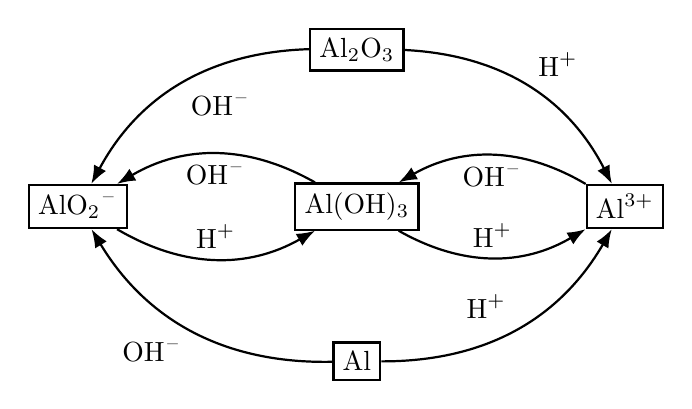
\begin{tikzpicture}[node distance=40pt, auto, thick]
		\node[draw] (Al2O3) {\ce{Al2O3}};
		\node[draw, below=of Al2O3] (AlOH) {\ce{Al(OH)3}};
		\node[draw, below=of AlOH] (Al) {\ce{Al}};
		\node[draw, right=60pt of AlOH] (Al3+) {\ce{Al^3+}};
		\node[draw, left=60pt of AlOH] (AlO2-) {\ce{AlO2-}};
		
		\draw[-Latex] (AlOH) [bend right] (AlO2-) edge node {\ce{H+}} (AlOH);
		\draw[-Latex] (AlO2-) [bend right] (AlOH) edge node {\ce{OH-}} (AlO2-);
		\draw[-Latex] (Al3+) [bend right] (AlOH) edge node {\ce{H+}} (Al3+);
		\draw[-Latex] (AlOH) [bend right] (Al3+) edge node {\ce{OH-}} (AlOH);
		\draw[-Latex] (Al3+) [bend left] (Al2O3) edge node {\ce{H+}} (Al3+);
		\draw[-Latex] (AlO2-) [bend right] (Al2O3) edge node {\ce{OH-}} (AlO2-);
		\draw[-Latex] (Al3+) [bend right] (Al) edge node {\ce{H+}} (Al3+);
		\draw[-Latex] (AlO2-) [bend left] (Al) edge node {\ce{OH-}} (AlO2-);
	\end{tikzpicture}
	\end{center}
\end{document}